\begin{figure}[!h]
	\centering
	\subbottom[positive\label{fig:posanchor}]
		{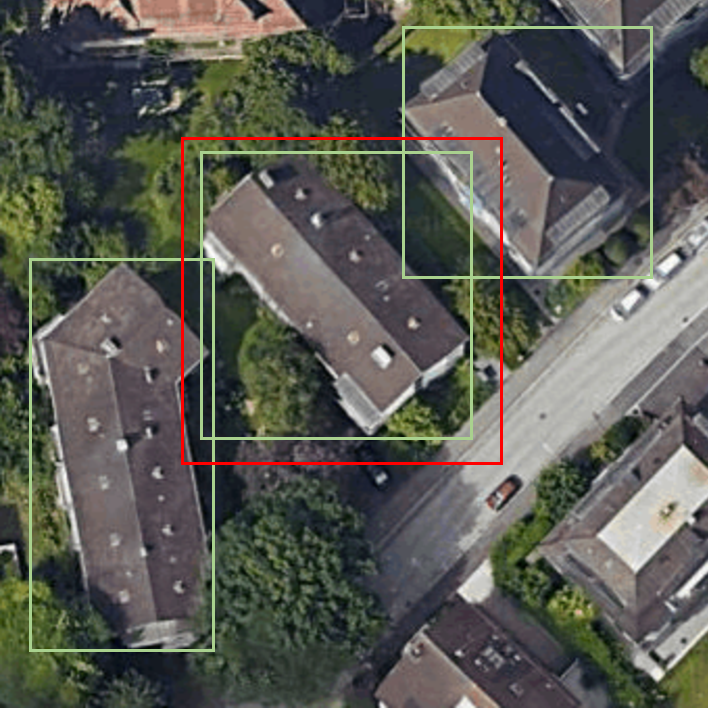
\includegraphics[width=\figfigfigfig\textwidth]{3-07-0.pdf}}
	\subbottom[natural\label{fig:natanchor1}]
		{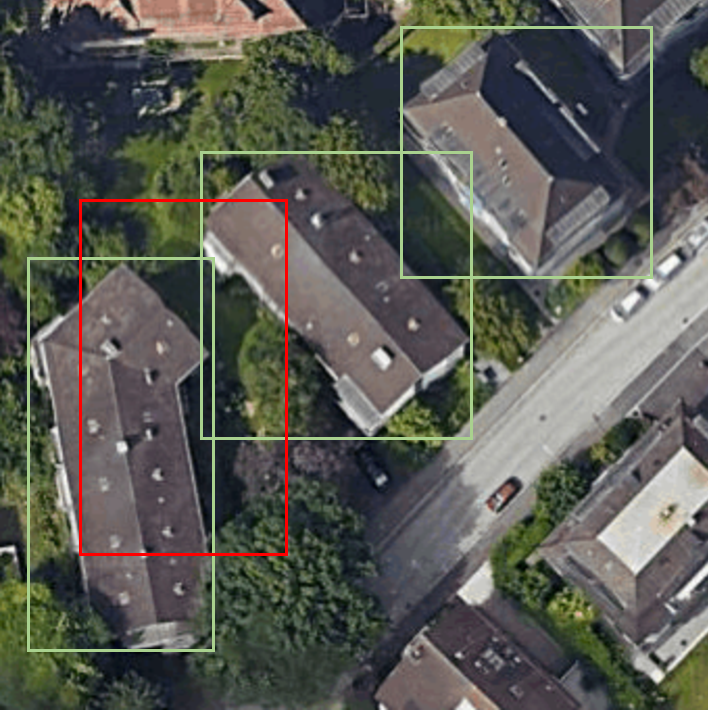
\includegraphics[width=\figfigfigfig\textwidth]{3-07-1.pdf}}
	\subbottom[natural\label{fig:natanchor2}]
		{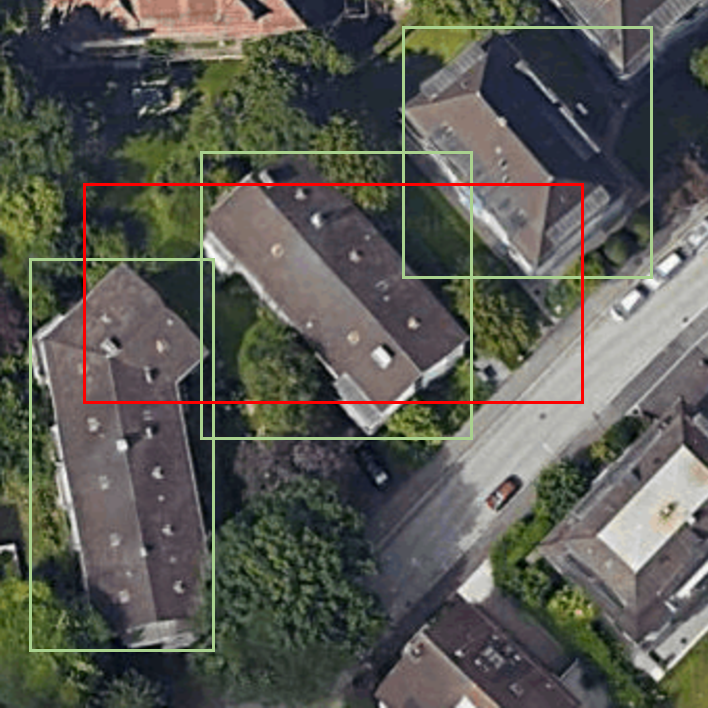
\includegraphics[width=\figfigfigfig\textwidth]{3-07-2.pdf}}
	\subbottom[negative\label{fig:neganchor}]
		{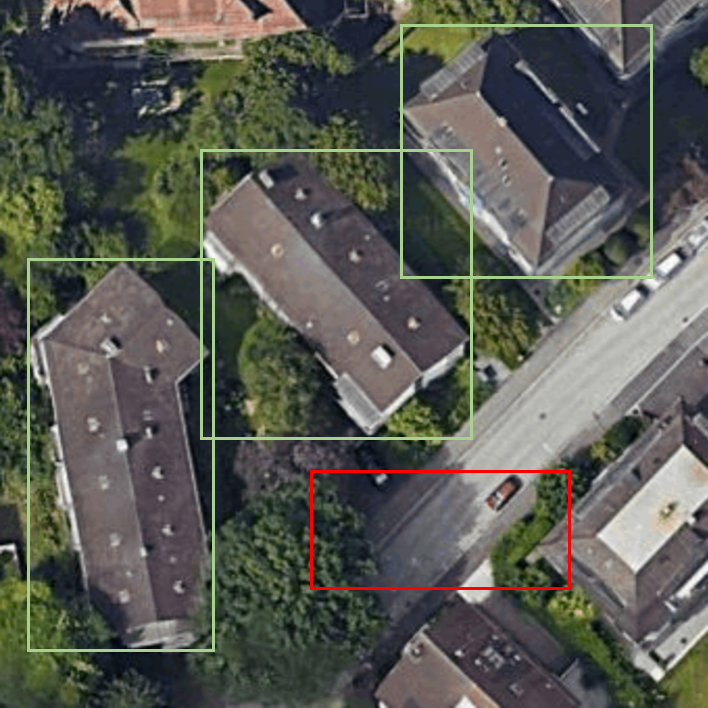
\includegraphics[width=\figfigfigfig\textwidth]{3-07-3.pdf}}
    \caption[Example anchors in an image with multiple RoIs]{Example anchors in an image with multiple RoIs. (a)--(d) show four possible anchors with each showing one. The red and light green rectangles refer to anchors and ground truth bounding boxes, respectively. The polarities of these anchors are also presented in the sub-captions, using the typical threshold.}
	\label{fig:eganchor}
\end{figure}